\subsection{Протокол Диффи~---~Хеллмана}\index{протокол!Диффи~---~Хеллмана|(}\index{схема!Диффи~---~Хеллмана|(}\label{section-protocols-diffie-hellman}
\selectlanguage{russian}

Первый алгоритм с открытым ключом был предложен Диффи и Хеллманом в работе 1976 года <<Новые направления в криптографии>> (\langen{Bailey Whitfield Diffie, Martin Edward Hellman, ``New directions in cryptography''},~\cite{Diffie:Hellman:1976}). Данный протокол, который также можно назвать \emph{схемой Диффи~---~Хеллмана}, стал первым, позволивший уменьшить требования к каналу связи для установления защищённого соединения без предварительного обмена ключами.

Протокол позволяет двум сторонам создать общий сеансовый ключ используя такой канал связи, который может прослушивать злоумышленник, но в предположении, что последний не может менять содержимое сообщений.

Пусть $p$ -- большое простое число\index{число!простое}, $g$ -- примитивный элемент группы $\Z_p^*$, ~ $y = g^x \bmod p$, причём $p, y, g$ известны заранее. Функцию $y=g^{x} \bmod p$ считаем однонаправленной, то есть вычисление функции при известном значении аргумента является лёгкой задачей, а её обращение (нахождение аргумента) при известном значении функции -- трудной.\footnote{Обратную функцию $x = \log_g y \bmod p$ называют функцией дискретного логарифма. В настоящий момент не существует быстрых способов вычисления такой функции для больших простых $p$.}

Протокол обмена состоит из следующих действий.

\begin{figure}
    \centering
    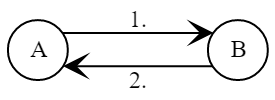
\includegraphics[width=0.5\textwidth]{pic/key_distribution-diffie-hellman}
    \caption{Обмен сообщениями в протоколе Диффи~---~Хеллмана\label{fig:key_distribution-diffie-hellman}}
\end{figure}

\begin{protocol}
    \item[(1)] Алиса выбирает случайное $2 \leq a \leq p - 1$
    \item[{}] $Alice \to \left\{ A = g ^ a \bmod p \right\} \to Bob$
    \item[(2)] Боб выбирает случайное $2 \leq b \leq p-1$
    \item[{}] Боб вычисляет сеансовый ключ $K = A ^ b \bmod p$
    \item[{}] $Bob \to \left\{ B = g ^ b \bmod p \right\} \to Alice$
    \item[(3)] Алиса вычисляет $K = B ^ a \bmod p$
\end{protocol}

Таким способом создан общий секретный сеансовый ключ $K$. За счёт случайного выбора значений $a$ и $b$ в каждом новом сеансе будет получен новой сеансовый ключ.

Протокол обеспечивает только генерацию новых сеансовых ключей (цель G10). В отсутствие третей доверенной стороны он не обеспечивает аутентификацию сторон (цель G1), а из-за отсутствия проходов с подтверждением владения ключом отсутствует аутентификация ключа (цель G8). Зато, так как протокол не использует длительные <<мастер>>-ключи, можно говорить о том, что он обладает свойством совершенной прямой секретности (цель G9).

Протокол можно использовать только с такими каналами связи, в которые не может вмешаться активный криптоаналитик. В противном случае протокол становится уязвим к простой атаке <<человек посередине>>\index{атака!<<человек посередине>>}.

\begin{figure}
    \centering
    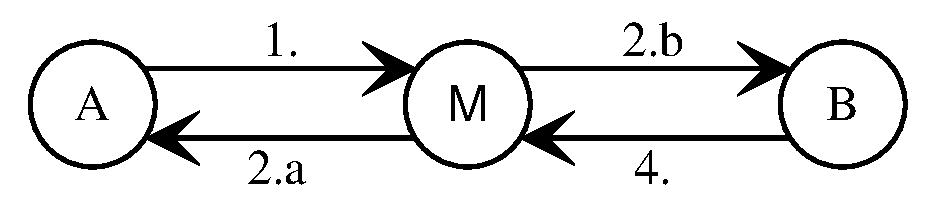
\includegraphics[width=0.67\textwidth]{pic/key_distribution-diffie-hellman-mitm}
    \caption{Схема взаимодействия участников в протоколе Диффи~---~Хеллмана при атаке <<человек посередине>>\label{fig:key_distribution-diffie-hellman-mitm}}
\end{figure}

\begin{protocol}
    \item[(1)] Алиса выбирает случайное $2 \leq a \leq p - 1$
    \item[{}] $Alice \to \left\{ A = g ^ a \bmod p \right\} \to Mellory~(Bob)$
    \item[(2)] Меллори выбирает случайное $2 \leq m \leq p-1$
    \item[{}] Меллори вычисляет сеансовый ключ для канала с Алисой
        \[K_{AM} = A ^ m \bmod p = g ^ {am} \bmod p\]
    \item[{}] $Mellory~(Alice) \to \left\{ M = g ^ m \bmod p \right\} \to Bob$
    \item[{}] $Mellory~(Bob) \to \left\{ M = g ^ m \bmod p \right\} \to Alice$
    \item[(3)] Алиса вычисляет сеансовый ключ для канала с Меллори (думая, что Меллори это Боб)
        \[K_{AM} = M ^ a \bmod p = g ^ { am } \bmod p\]
\pagebreak
    \item[(4)] Боб выбирает случайное $2 \leq b \leq p-1$
    \item[{}] Боб вычисляет сеансовый ключ для канала с Меллори (думая, что Меллори это Алиса)
        \[K_{BM} = M ^ b \bmod p = g ^ { bm } \bmod p\]
    \item[{}] $Bob \to \left\{ B = g ^ b \bmod p \right\} \to Mellory~(Alice)$
    \item[(5)] Меллори вычисляет сеансовый ключ для канала с Бобом
        \[K_{BM} = B ^ m \bmod p = g ^ { bm } \bmod p\]
\end{protocol}

В результате Алиса и Боб получили новые сеансовые ключи, но <<защищённый>> канал связи установили не с друг с другом, а со злоумышленником, который теперь имеет возможность ретранслировать или изменять все передаваемые сообщения между Алисой и Бобом.

Протокол Диффи~---~Хеллмана отличается от большей части протоколов распространения ключей из-за того, что не использует другие криптографические примитивы (функции шифрования, электронно-цифровой подписи или хеширования), но сам по себе является в некотором смысле криптографическим примитивом для построения более сложных протоколов. Он обеспечивает генерацию случайного числа в распределённой системе без доверенного центра. Причём ни одна из сторон не может заставить другую сторону использовать старый сессионный ключ, в отличие от, например, протокола Yahalom\index{протокол!Yahalom} из раздела~\ref{section-protocols-yahalom}.

Протокол можно изменить таким образом, чтобы вместо мультипликативной группы простого умножения использовать аддитивную группу сложения точек эллиптической кривой (см. раздел~\ref{section-math-ec-groups}). В этом случае стороны по прежнему будут выбирать некоторые случайные целые числа, но не возводить генератор-число в степень, а умножать генератор-точку на загаданное число.

\begin{protocol}
    \item[(0)] Стороны договорились о группе точек эллиптической кривой $\group{E}$, её циклической подгруппе $\group{G}$ мощности $n = \| \group{G} \|$ и генераторе $G$ группы $\group{G}$ (или хотя бы достаточно большой подгруппы группы $\group{G}$).
    \item[(1)] Алиса выбирает случайное $2 \leq a \leq n - 1$
    \item[{}] $Alice \to \left\{ A = a \times G \right\} \to Bob$
    \item[(2)] Боб выбирает случайное $2 \leq b \leq n - 1$
    \item[{}] Боб вычисляет точку $K = b \times A$
    \item[{}] $Bob \to \left\{ B = g \times G \right\} \to Alice$
    \item[(3)] Алиса вычисляет точку $K = a \times B$
\end{protocol}

В качестве нового сессионного ключа стороны могут выбрать, например, первую координату найденной точки $K$.

\index{протокол!Диффи~---~Хеллмана|)}\index{схема!Диффи~---~Хеллмана|)}